\documentclass{beamer}

\usetheme{default}
\usepackage{fancyvrb,relsize}
\usepackage{slashbox}
\usetheme{Warsaw}
\usepackage{amsmath}
\usepackage{bbding}
\usepackage{courier}
\usepackage{enumerate}
\setbeamertemplate{itemize items}[circle]
\usepackage{graphicx}
\usepackage{listings}
\usepackage{fancybox}
\usepackage[normalem]{ulem}
% \usepackage{graphics}
%\usepackage{epstopdf}

\mode<presentation>
{
\setbeamertemplate{footline}
{\rightline{\insertframenumber/\inserttotalframenumber}}
}

\title{A Framework for \\Automatic OpenMP Code Generation
 }
\author{\textbf{Raghesh A} (CS09M032)\\\ \\ Guide: \textbf{Dr.~Shankar~Balachandran}}
\date{May 2nd, 2011}

\begin{document}

% slide
\begin{frame}
\titlepage
\end{frame}

% slide
\begin{frame}{Outline}
\begin{itemize}
\item The Framework
\item An Example
\item Necessary Background
\item Polyhedral Model
\item SCoP - Static Control Part
\item LLVM in Polly
\item Polly
\item OpenMP Code Generation in Polly
\item Experimental Results
\item Conclusion 
\item Future Work
\end{itemize}
\end{frame}

\begin{frame}{The Framework}
\begin{figure}
\begin{center}
  \includegraphics[width=1\textwidth]{images/framework.eps}
  %\caption{Transformation in polyhedral model}
\end{center}  
\end{figure}
\end{frame}


\begin{frame}{An Example}
\begin{columns}[t]
\only<1>{
	\column{.7\textwidth}
	\begin{block}{Source code}
	{\lstinputlisting{code/a.c}}
	\end{block}
}
\only<2>{
	\column{.5\textwidth}
	\begin{block}{LLVM-IR Sequential}
	%{\tiny\lstinputlisting{code/a.ll}}
	\input{code/a.ll.tex}
	\end{block}
}
\only<2>{
	\column{.5\textwidth}
	\begin{block}{LLVM-IR Sequential}
	\input{code/a.ll.1.tex}
	\end{block}
}
\only<3>{
	\column{.7\textwidth}
	\begin{block}{Source code with OpenMP pragmas}
	{\lstinputlisting{code/a.gcc.c}}
	\end{block}
}
\only<4>{
	\column{.5\textwidth}
	\begin{block}{LLVM-IR Manual}
	\input{code/a.gcc.ll.tex}
	\end{block}
}
\only<4>{
	\column{.5\textwidth}
	\begin{block}{LLVM-IR Manual}
	\input{code/a.gcc.ll.1.tex}
	\end{block}
}
\only<5>{
	\column{.5\textwidth}
	\begin{block}{LLVM-IR Automatic}
	\input{code/a.polly.ll.tex}
	\end{block}
}
\only<5>{
	\column{.5\textwidth}
	\begin{block}{LLVM-IR Automatic}
	\input{code/a.polly.ll.1}
	\end{block}
}
\end{columns}
\end{frame}

% slide
\begin{frame}{Necessary Background}
\begin{itemize}
\item Parallelism in programs
	\begin{itemize}
	\item Parallelism and locality
	\item Realizing parallelism
	\end{itemize}
\item Auto parallelization
\item The polyhedral model
\item LLVM
\item Polly \\
\end{itemize}
\pause
\ \\
\ \\
\ \\	
\begin{center}
{\textbf {Workdone: \color{red}{"OpenMP Code Generation in Polly"}}}
\end{center}
\end{frame}


\begin{frame}{The Polyhedral Model}
\begin{itemize}
\item Examples for transformations with polyhedral model
	\begin{itemize}
	\item Transformation for improving data locality
	\begin{columns}[t]
	\pause
		\column{.5\textwidth}
		\begin{block}{ }
	{\tiny\lstinputlisting{listing1.tex}}
		\end{block}


	\pause
		\column{.5\textwidth}
		\begin{block}{ }
	{\tiny\lstinputlisting{listing2.tex}}
		\end{block}
	\end{columns}
	\ \\
	\pause
	\item Scalar expansion
	\pause
	\begin{columns}[t]
		\column{.5\textwidth}
		\begin{block}{ }
		{\tiny\lstinputlisting{listing3.tex}}
		\end{block}
	\pause
		\column{.5\textwidth}
		\begin{block}{ }
		{\tiny\lstinputlisting{listing4.tex}}
		\end{block}
	\end{columns}
        \pause
	\begin{columns}
	%\column{.25\textwidth}
	\column{0.5\textwidth}
		\begin{block}{ }
		{\tiny\lstinputlisting{listing5.tex}}
		\end{block}
		\end{columns}
	\end{itemize}
\end{itemize}
\end{frame}


\begin{frame}{Polyhedral Representation of Programs}
\begin{itemize}
\item Iteration domain
\item Schedule
\item Access function
\end{itemize}

\pause
\color{red}{\textbf{Dynamic instances of each statement is represented as an integer point in statement's polyhedron}}

\pause
\begin{itemize}
\item Why not AST?
	\begin{itemize}
	\item Dynamic instances of statements not captured
	\item Rigid data structure
	\item Less expressive than polyhedral model
	\end{itemize}

\pause	
\item Transformation in polyhedral model 
\end{itemize}
\begin{figure}
\begin{center}
  \includegraphics[width=1\textwidth]{images/poly_steps.eps}
  %\caption{Transformation in polyhedral model}
  \label{fig:iter1}
\end{center}  
\end{figure}

\end{frame}

\begin{frame}[shrink]{Iteration Domain}
\begin{columns}[t]
	\column{.5\textwidth}
	\begin{block}{ }
	{\tiny\lstinputlisting{listing6.tex}}
	\end{block}
	
	\column{.5\textwidth}
	\begin{block}{ }
	{\tiny\lstinputlisting{listing7.tex}}
	\end{block}
	\end{columns}
\pause
Iteration domain for {\textbf S1} is 
$D_{S1}\ =\ \{(i,j)\ \epsilon\ Z^2\ |\ 2\ \leq\ i\ \leq\ N\ \wedge\ 2\ \leq\ j\ \leq\ N\}$
\linebreak\linebreak
Iteration domain for {\textbf S2} is 
$D_{S2}\ =\ \{(i,j)\ \epsilon\ Z^2\ |\ 2\ \leq\ i\ \leq\ 6\ \wedge\ 2\ \leq\ j\ \leq\ 6\ \wedge\ i\ \leq\ j\}$
\pause
\begin{figure}
\begin{center}
  \includegraphics[height=5cm,width=5cm]{images/iter1.eps}
  \caption{Graphical representation of iteration domain(S2)}
  \label{fig:iter1}
\end{center}  
\end{figure}
\end{frame}

\begin{frame}{Schedule}

\only<1,2,3,4> {
\begin{itemize}
\item Scattering function
\end{itemize}

\begin{block}{ }
{\tiny\lstinputlisting{listing8.tex}}
\end{block}
{\textbf{\color{red}{Assigning execution date for each statement instance. Instances with same execution dates can be run in parallel}}}
}
\only<2,3,4> {
Examples: \\
$\phi_{S3}(i,j) = (i,j)$ \pause\ \ \ $\phi^{'}_{S3}(i,j) = (j,i)$
$\phi^{''}_{S3}(i,j) = \{(i,jj,j):jj\ mod\ 4\ =\ 0\ \wedge\ jj\ \leq\ j\ <\ jj\ +\ 4\}$
}

\only<3> {
\begin{block}{Code generated for $\phi^{'}_{S3}$}
{\tiny\lstinputlisting{listing9.tex}}
\end{block}
}

\only<4> {
\begin{block}{Code generated for $\phi^{'}_{S3}$ o $\phi^{''}_{S3}$}
{\tiny\lstinputlisting{listing9.1.tex}}
\end{block}
}

\only<3> {
Loops are \textbf{\color{red}{interchanged}} here by applying this transformation
}
\only<4> {
Loops are \textbf{\color{red}{stripmined}} here by applying this transformation
}

\end{frame}

\begin{frame}{Access Function}
A[i+j][i+N]
\linebreak\linebreak
Array access function: $F_A(i,j) = (i+j,i+N)$ 
\linebreak\linebreak
{\textbf {\color{red}{Change array access function for better locality}}} \\
\end{frame}

\begin{frame}{SCoP - Static Control Part}
\begin{block}{Example for SCoP}
{\lstinputlisting{listing14.tex}}
\end{block}

\begin{itemize}
\item Structured control flow
	\begin{itemize}
	\item Regular for loops
	\item Conditions
	\end{itemize}
\item Affine expressions in:
	\begin{itemize}
	\item Loop bounds
	\item Conditions
	\item Access functions
	\end{itemize}
\item Side effect free(Pure functions)
\end{itemize}

\end{frame}

\begin{frame}{LLVM in Polly}
\begin{itemize}
\item LLVM (Low Level Virtual Machine)
	\begin{itemize}
	\item Framework for implementing compilers
	\item Common low level code representation
	\item Lifelong analysis and transformation of programs
	\end{itemize}
\item LLVM relaxes SCoP constraints -$>$ more SCoPs are detected
	\begin{itemize}
	\item \sout{Regular for loops} -$>$ Anything that acts like a regular for loop
	\item \sout{Affine expressions} -$>$ Expressions that calculates an affine result
	\item Side effect \sout{free} known
	\item Memory access through \sout{arrays} arrays + pointers
	\end{itemize}
\item Independent of programming language
\end{itemize}
\end{frame}

\begin{frame}{Polly}
\begin{itemize}
\item Polly (Polyhedral Optimization in LLVM)
	\begin{itemize}
	\item Implementing Polyhedral Optimization in LLVM
	\item Effort towards Auto Parallelism in programs.
	\end{itemize}
\item Implementation
	\begin{itemize}
	\item LLVM-IR to polyhedral model
			\begin{itemize}
			\item Region-based SCoP detection
			\item Semantic SCoPs
			\end{itemize}
	\item Polyhedral model
		\begin{itemize}
		\item The integer set library
		\item Polyhedral transformations
		\item Export/Import
		\end{itemize}
	\item Polyhedral model to LLVM-IR
	\end{itemize}
\item Related work
	\begin{itemize}
	\item gcc Graphite
	\end{itemize}
\end{itemize}
\end{frame}

\begin{frame}{Polly}
\begin{figure}
  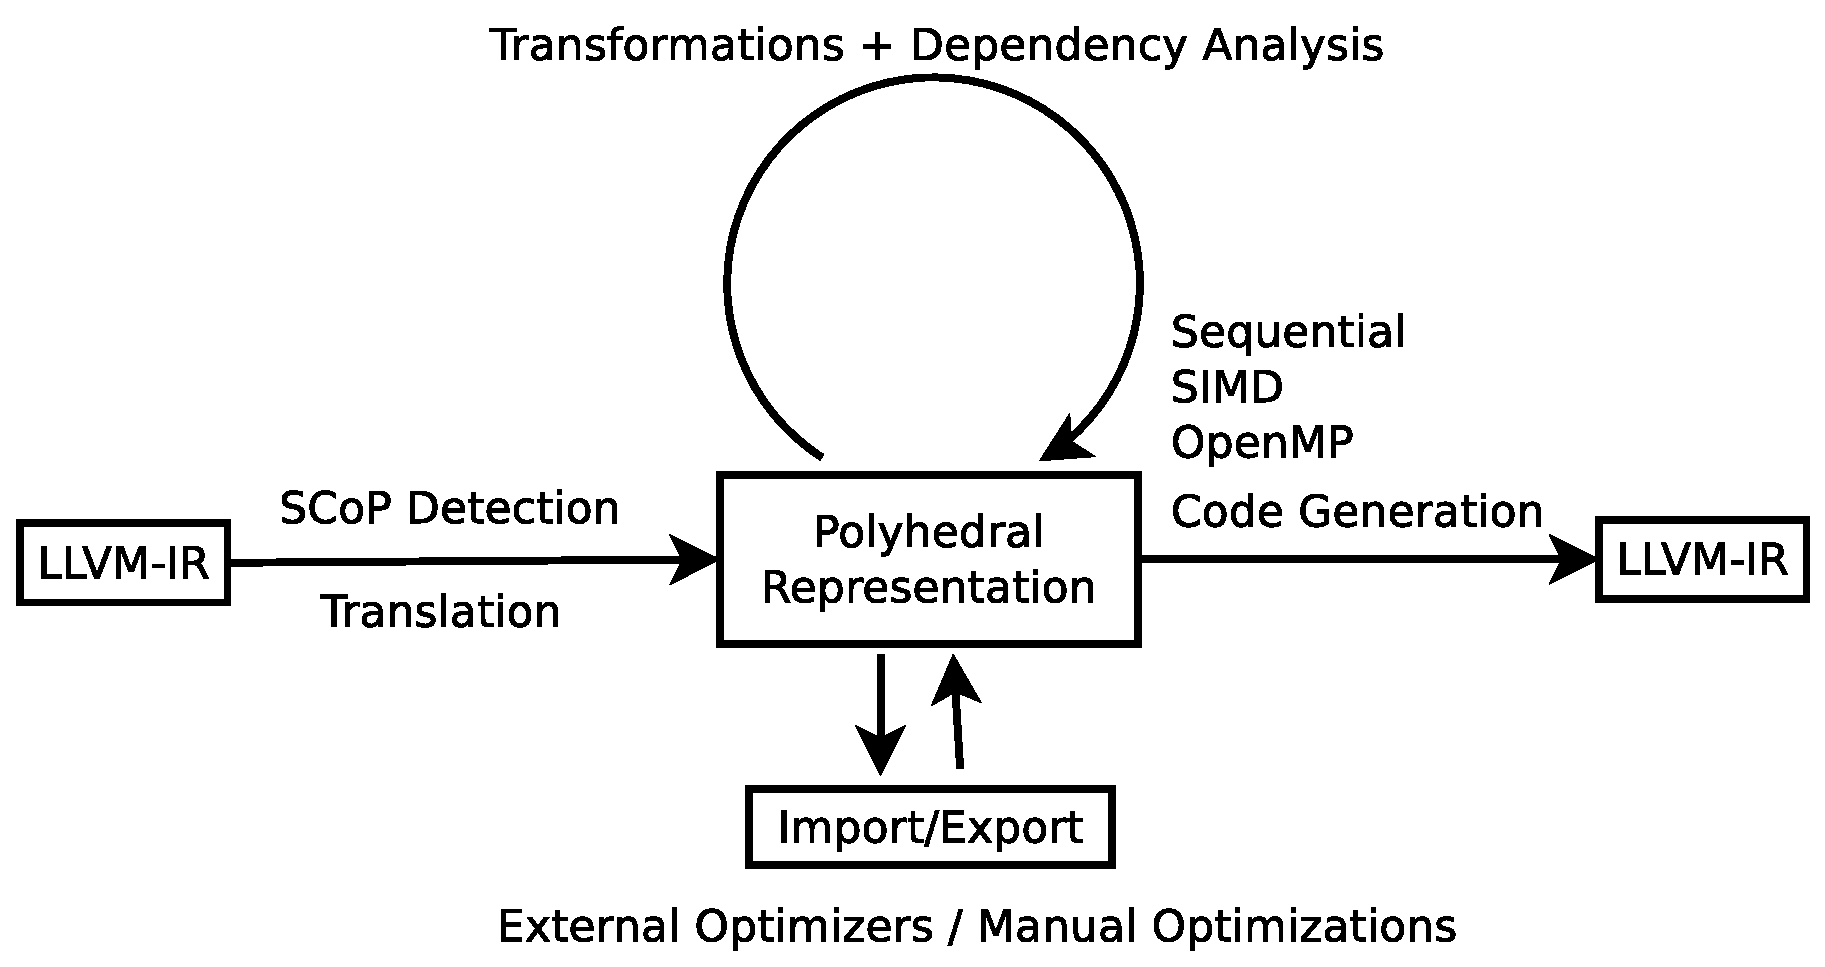
\includegraphics[width=1\textwidth]{images/architecture.eps}
  \caption{Architecture of Polly}
  \label{fig:arch}
\end{figure}
\end{frame}

\begin{frame}{OpenMP Code Generation in Polly}
\begin{figure}
\begin{center}
  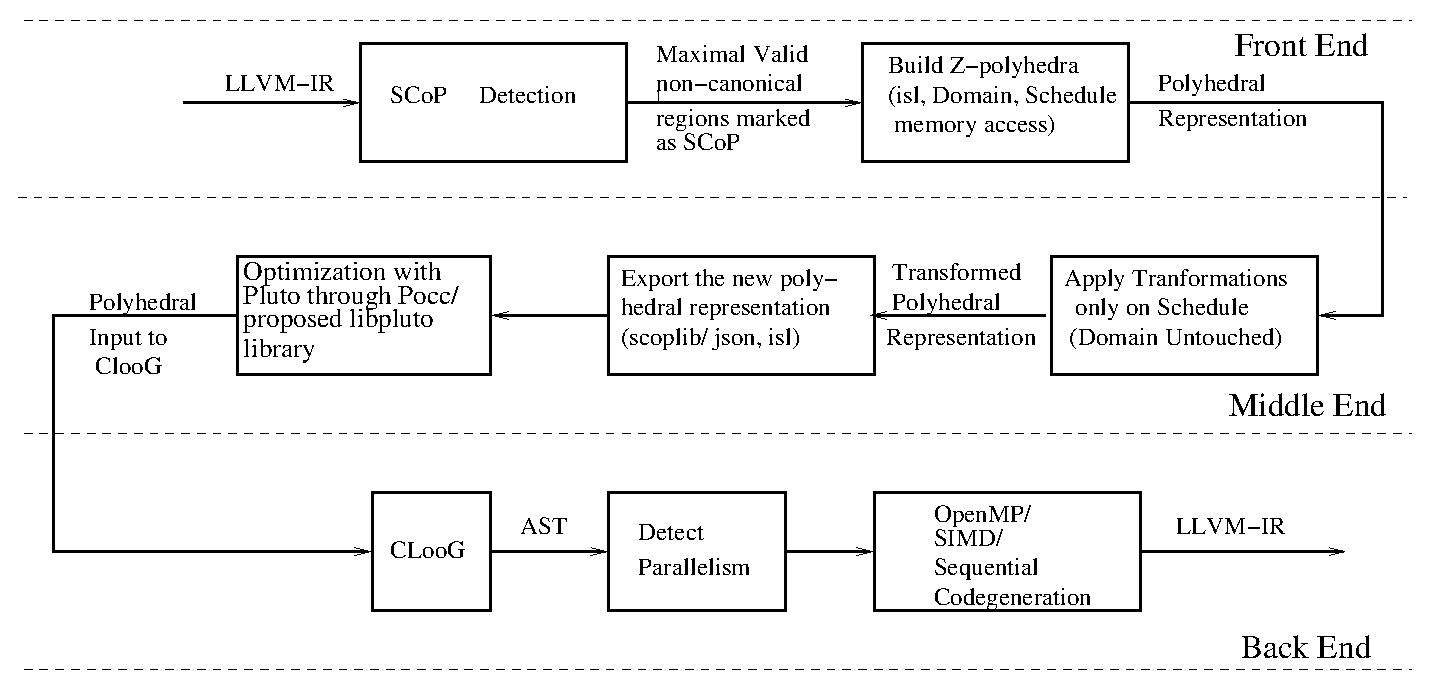
\includegraphics[width=1\textwidth]{images/detailedarch.eps}
  \caption{Detailed control flow in Polly}
  \label{detailed}
\end{center}
\end{figure}
\end{frame}


\begin{frame}{OpenMP Code Generation in Polly}
\begin{itemize}
\item Code generation pass in Polly
\item Detecting parallelism in Polly
\item Generating OpenMP library calls
\end{itemize}

\begin{block}{ }
{\footnotesize\lstinputlisting{listing10.tex}}
\end{block}
\end{frame}

\begin{frame}{OpenMP Code Generation in Polly}
\begin{figure}
  %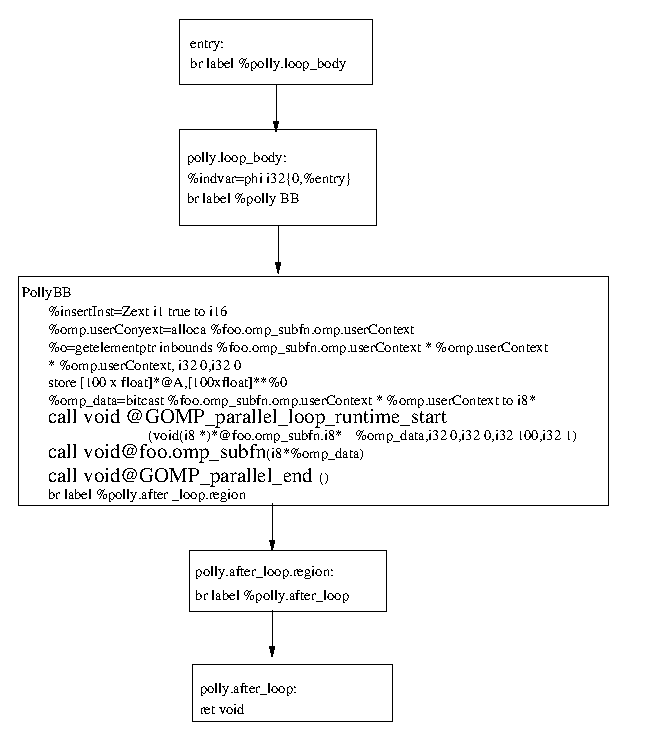
\includegraphics[width=1\textwidth]{images/ompcalls.eps}
  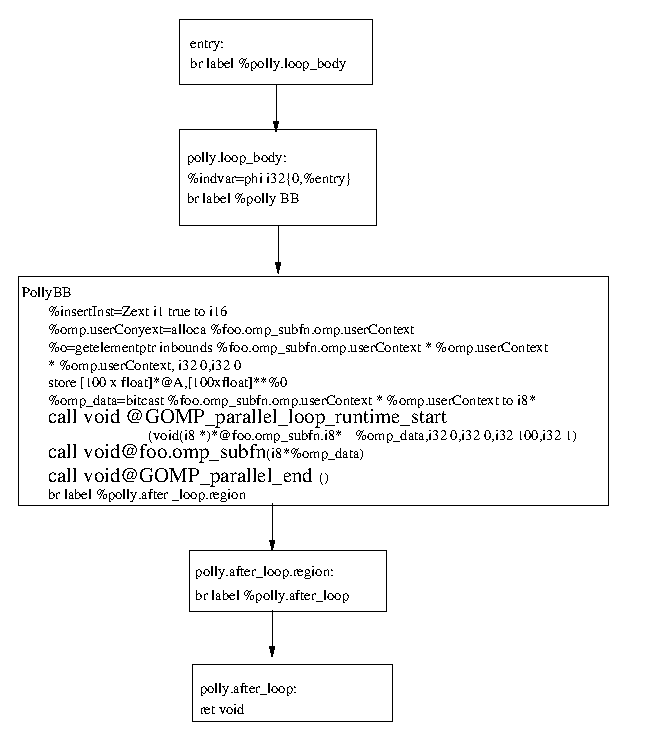
\includegraphics[width=1\textwidth]{images/ompcalls.eps}
  \caption{CFG showing sequence of OpenMP library calls}
  \label{fig:openmp_cfg}
\end{figure}
\end{frame}


\begin{frame}{OpenMP Code Generation in Polly}
\begin{itemize}
\item Support for inner loops

\begin{block}{ }
{\footnotesize\lstinputlisting{listing11.tex}}
\end{block}
Surrounding induction variables and parameters need to be passed to the subfunction
\pause
\item Dealing with memory references
\begin{block}{ }
{\footnotesize\lstinputlisting{listing12.tex}}
\end{block}
	\begin{itemize}
	\item Adding and extracting memory references
	\end{itemize}
\end{itemize}
\end{frame}


\begin{frame}{OpenMP Code Generation in Polly}
\begin{itemize}
\item Enabling OpenMP code generation in Polly
\begin{block}{ }
{\tiny\lstinputlisting{listing13.tex}}
\end{block}
\item OpenMP testcases
	\begin{itemize}
	\item Polly follows LLVM testing infrastructure
	\end{itemize}
\end{itemize}
\end{frame}

\begin{frame}[shrink]{Testing}
\begin{itemize}
\item GCC Compile farm
\end{itemize}

\pause

\begin{block}{A simple test case}
{\tiny \lstinputlisting{code/c.c}}
\end{block}
\pause
\begin{table}[h]
\begin{center}
{\footnotesize
\begin{tabular}{| l | p{2cm} | p{2cm} | p{2cm} | p{2cm} |}
\hline
& \textbf{Serial Execution} & \textbf{Automatic Parallelization(Polly)} & \textbf{Manual Parallelization(GCC)} \\ \hline
\textbf{Intel Core 2 Duo}(32 Bit OS)& 9.509s & 4.852s & 4.835s \\ \hline
\textbf{Intel Core 2 Duo}(64 Bit OS)& 6.40s  & 3.32s & 3.50s\\ \hline
\textbf{Intel Core i5}(64 Bit OS)   & 6.96s  & 3.78s & 3.75s\\ \hline
\textbf{AMD Engineering Sample(24 Core)}(64 Bit OS)   & 17.039s & 0.757s & 0.796s\\
\hline
\end{tabular}
}
\end{center}
\caption{Performance Comparison}
\end{table}

\color{red}{\textbf{Automatic OpenMP code generation in Polly gives similar results as GCC with OpenMP pragmas}}

\end{frame}
\begin{frame}{Testing with PolyBench}
\begin{itemize}
\item PolyBench \\
	\ \ \ Benchmarks from
	\begin{itemize}
	\item linear algebra
	\item datamining
	\item stencil computation
	\item solver and manipulation algorithms operating on matrices
	\end{itemize}
\end{itemize}
\end{frame}

\begin{frame}{Experimental Results}
\begin{figure}
\begin{center}
  \includegraphics[height=7cm]{images/2core32bit.eps}
  \caption{Performance comparison(2 core 32 bit)}
  \label{fig:2core1}
\end{center}
\end{figure}
\end{frame}

\begin{frame}{Experimental Results}
\begin{figure}
\begin{center}
  \includegraphics[height=7cm]{images/2core64bit.eps}
  \caption{Performance comparison(2 core 64bit)}
  \label{fig:2core2}
\end{center}
\end{figure}
\end{frame}

\begin{frame}{Experimental Results}
\begin{figure}
\begin{center}
  \includegraphics[height=7cm]{images/10core64bit.eps}
  \caption{Performance comparison(10-core 64 bit)}
  \label{fig:10core}
\end{center}
\end{figure}
\end{frame}

\begin{frame}[shrink]{Improving seidel's performance}

\begin{itemize}
\item {\textbf{\color{red}{Polly + Pluto + OpenMP + OMP\_SCHEDULE=guided}}}
\end{itemize}

\begin{table}[h]
\begin{center}
{\footnotesize
\begin{tabular}{| l | p{2cm} | p{2cm} | p{2cm} | p{2cm} |}
\hline
& \textbf{Serial Execution} & \textbf{Polly + OpenMP} & \textbf{Polly + PLUTO + OpenMP} \\ \hline
\textbf{2 Core 32 Bit} & 0.417174s & 0.591673s & 0.348909s \\ \hline
\textbf{2 Core 64 Bit} & 0.310160s  &  0.459641s & 0.254605s\\ \hline
\end{tabular}
}
\end{center}
\caption{Performance improvement of seidel}
\label{table:seidel}
\end{table}

\begin{table}[h]
\begin{center}
{\footnotesize
\begin{tabular}{| c | p{2cm} | p{2cm} | p{2cm} | p{2cm} |}
\hline
\backslashbox {No of threads}{Chunk size} &                 \textbf{512}  & \textbf{256}  & \textbf{128}  \\ \hline
  \textbf{default} & 12.930170s &  11.254353s   &  37.003882s   \\ \hline
  \textbf{10}      & 15.433336s &  14.657253s   &  14.518356s   \\ \hline
  \textbf{5}       & 14.002886s &  12.283284s   & 14.018281s    \\ \hline
  \textbf{2}       & 16.649145s &  18.778266s   & 18.013177s    \\ \hline
\end{tabular}
}
\end{center}
\caption{Performance of seidel with different OpenMP parameters}
\label{table:seidel:10core}
\end{table}

\end{frame}


\begin{frame}{Conclusion}
\begin{itemize}
\item Conclusion
	\begin{itemize}
	\item Burden of manual annotation eliminated
	\item More SCoP coverage
	\item LLVM's pre-optimzation passes helps a lot
	\item Enough space for further improvement -$>$ all are welcome to contribute
	\end{itemize}
\end{itemize}
\end{frame}
\begin{frame}[shrink]{Future Work}
\begin{itemize}
\item Support for memory access transformations in Polly {\color{red}{(Planned for GSOC 2011)}}
	\begin{itemize}
	\item Transformation on access function also
	\end{itemize}
\item Increasing coverage of Polly
	\begin{itemize}
	\item Increasing SCoP coverage
	\item Increasing the system coverage
	\end{itemize}
\item Integrating profile guided optimization into Polly
\end{itemize}
	\begin{columns}[t]
\only<1,2> {	
	%\pause
		\column{.5\textwidth}
		\begin{block}{Not a valid SCoP}
	{\tiny\lstinputlisting{listing15.tex}}
		\end{block}
}

\only<1> {	
		\column{.5\textwidth}
}
\only<2> {	
%	\pause
		\column{.5\textwidth}
		\begin{block}{With profiling observed b = 2 most of the times}
	{\tiny\lstinputlisting{listing16.tex}}
		\end{block}
}
	\end{columns}

\only<3> {	
%	\pause
\begin{block}{If N is small no need to detect this as a SCoP}
{\tiny\lstinputlisting{listing17.tex}}
\end{block}
}

\end{frame}

\begin{frame}{Publication}
\vspace{-0.3cm}

\begin{enumerate}
\item Tobias Grosser, Hongbin Zheng, \textbf{Raghesh Aloor}, Andreas Simb{\"u}rger, Armin {G}r{\"o}{\ss}linger and Louis-No{\"e}l Pouchet 
  Polly - Polyhedral optimization in LLVM {\em
  IMPACT 2011(First International workshop on PolyhedrAl Compilation Techniques as part of CGO 2011)}, Chamonix, France.
\end{enumerate}

\end{frame}


\begin{frame}{What Did I Achieve?}
\begin{itemize}
\item An interesting area to work
\item A platform to strengthen my knowledge
\item An opportunity to improve my mathematical skills
\item Skill to work in a collaborative environment, especially in free software way
\end{itemize}
\end{frame}

\begin{frame}{\ }
\begin{center} \textbf{\emph{Questions????}} \end{center}
\end{frame}

\begin{frame}{\ }
\begin{center} \textbf{\emph{THANK YOU}} \end{center}
\end{frame}
\end{document}
